\section{Workflow Demonstration}\label{workflow-demonstration}

To provide a clearer understanding of how the VV library operates in a
real-world scenario, this section walks through a complete workflow of
data visualization automation. The illustration starts from obtaining
data from a specific data source to rendering a chart and ultimately
deploying it to a Miro board and Google Drive.

\subsection{Stage 1: Data Retrieval}\label{stage-1-data-retrieval}

In this example, we consider healthcare data obtained from Google
Spreadsheets, which serve as our data source (see Figure \ref{fig:sheets_folder}). The
spreadsheets are organized into named ranges and contain essential
metrics for Cox Proportional Hazards Models (see Figure \ref{fig:ss}). These
metrics include hazard ratios along with their corresponding confidence
intervals for various covariates. The VV library leverages the
GoogleSpreadsheetDatasetBuilder class to fetch this data, which is then
transformed into a format suitable for chart rendering.

\begin{figure}[ht]
  \centering
  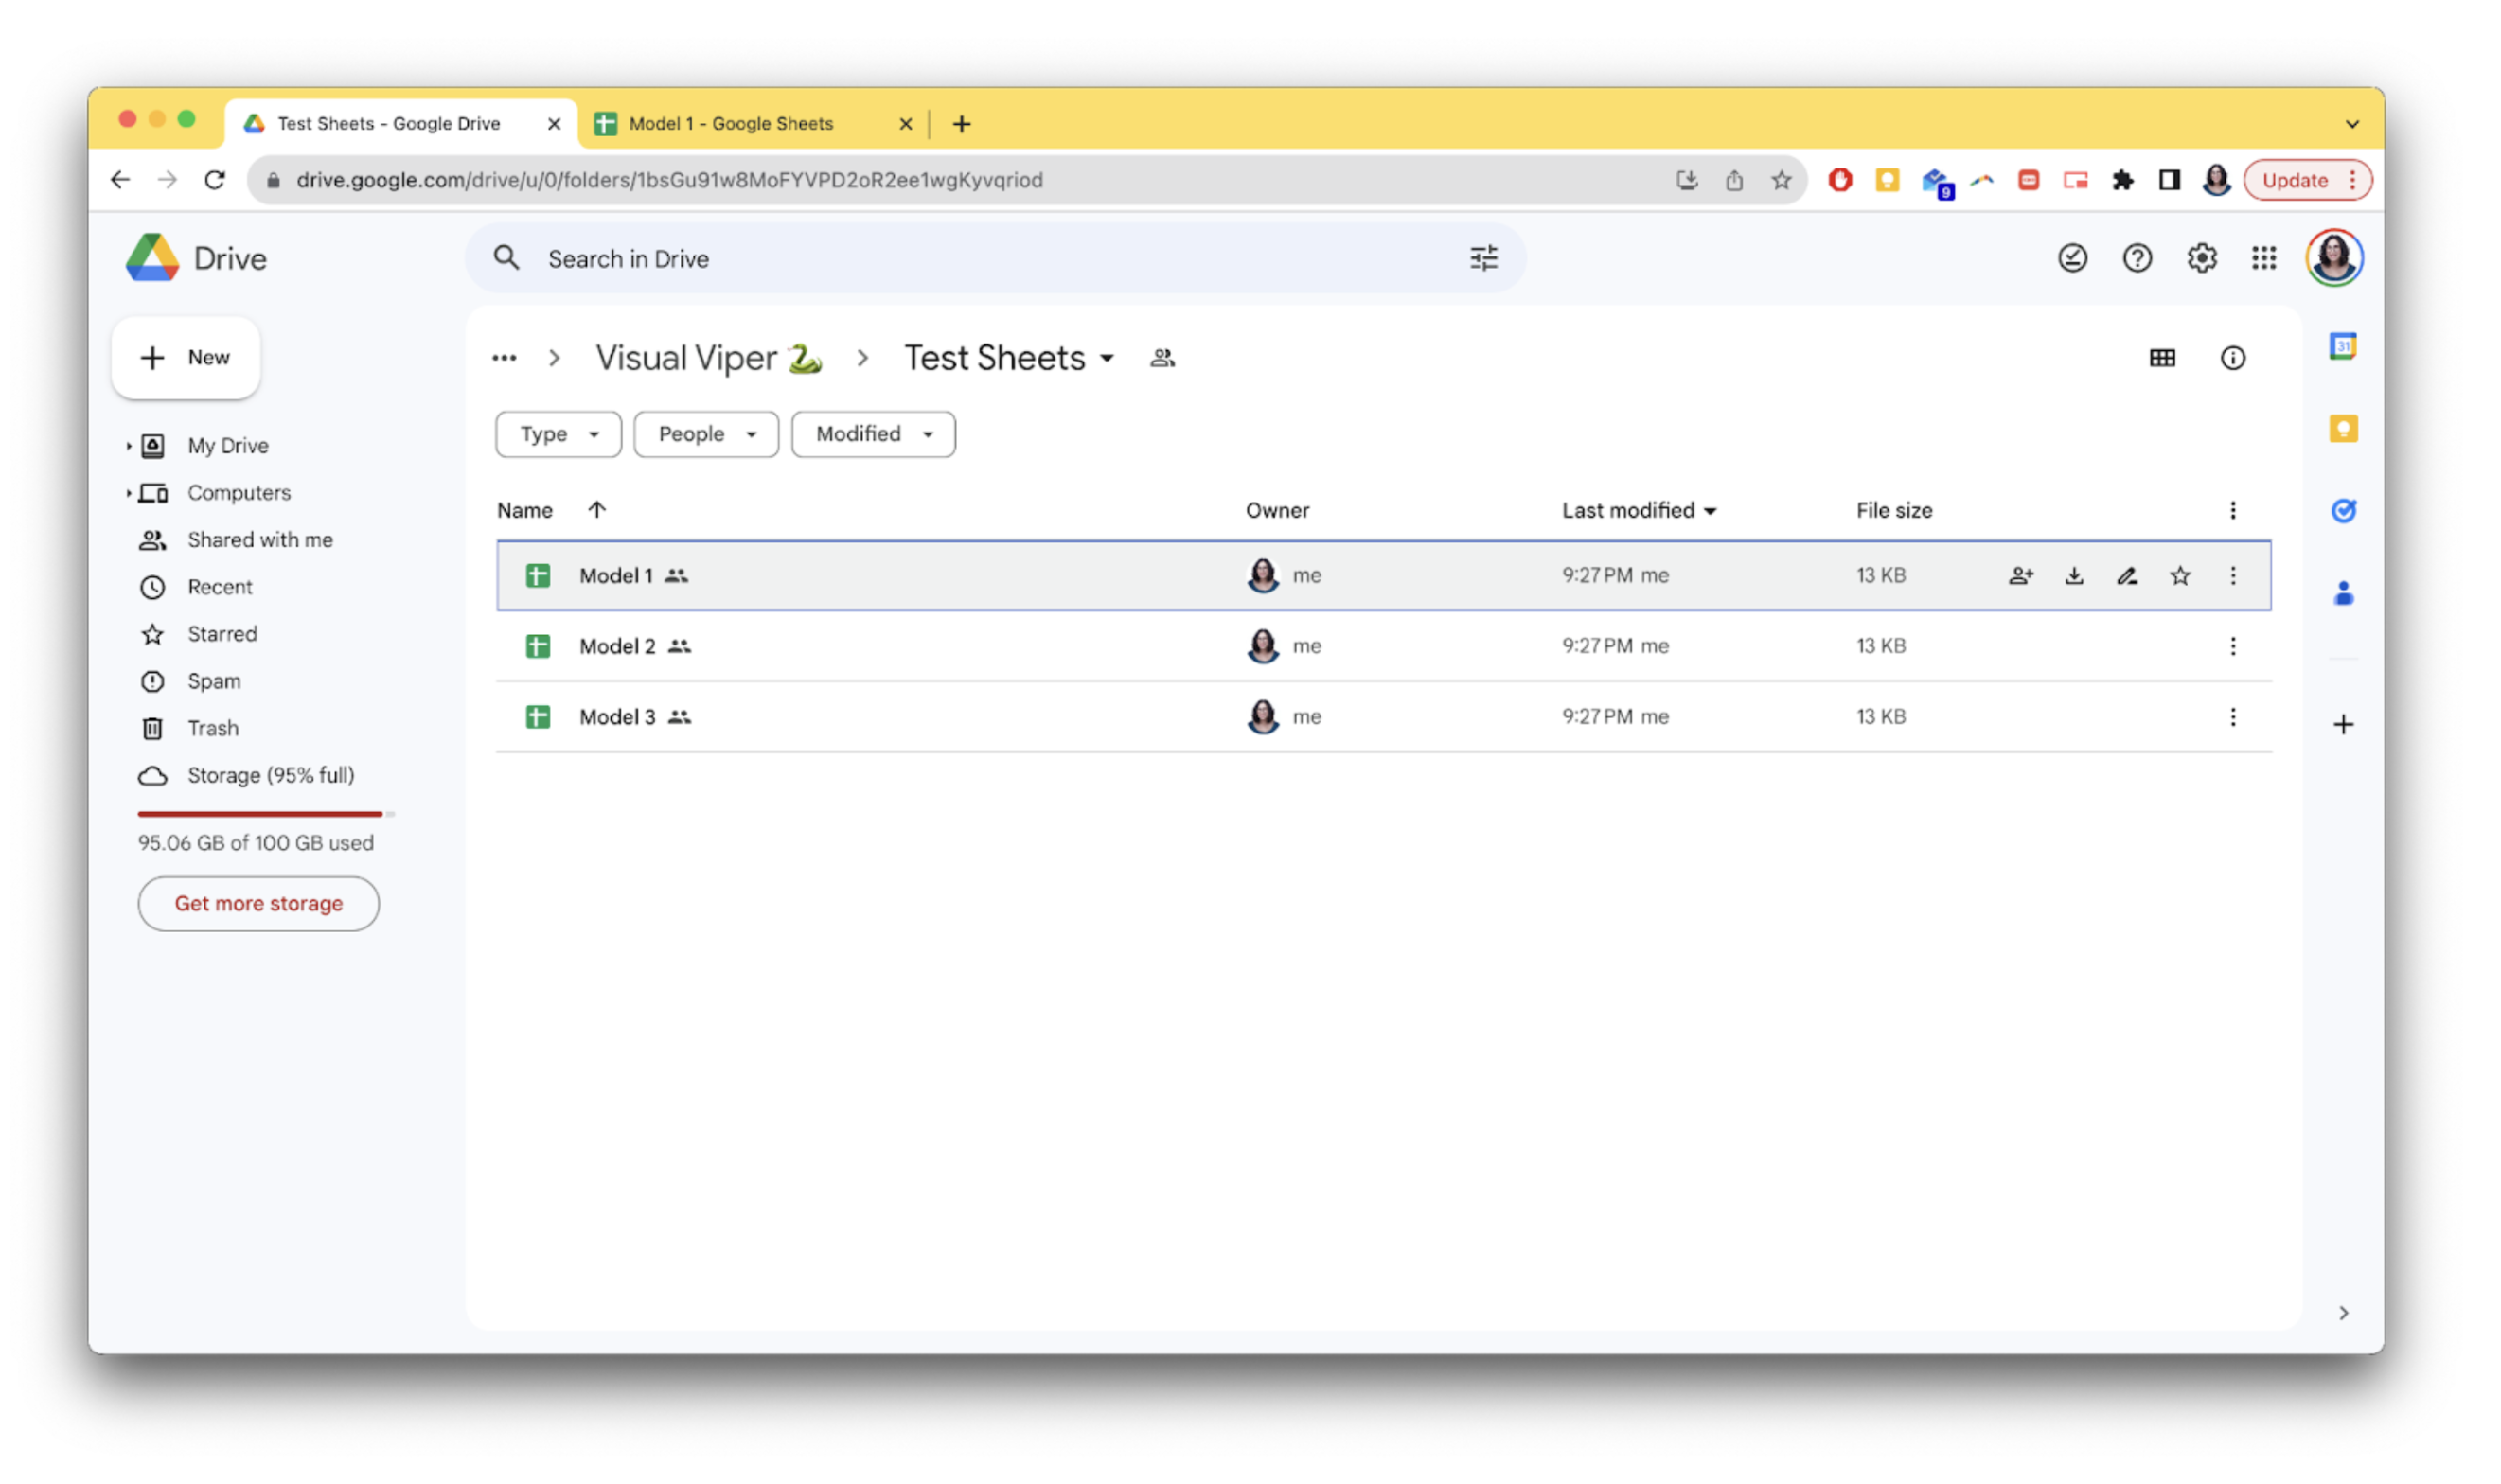
\includegraphics[width=\textwidth]{media/fig13.png}
  \caption{Folder Containing Google Spreadsheets for the example.}
  \label{fig:sheets_folder}
\end{figure}

\begin{figure}[ht]
  \centering
  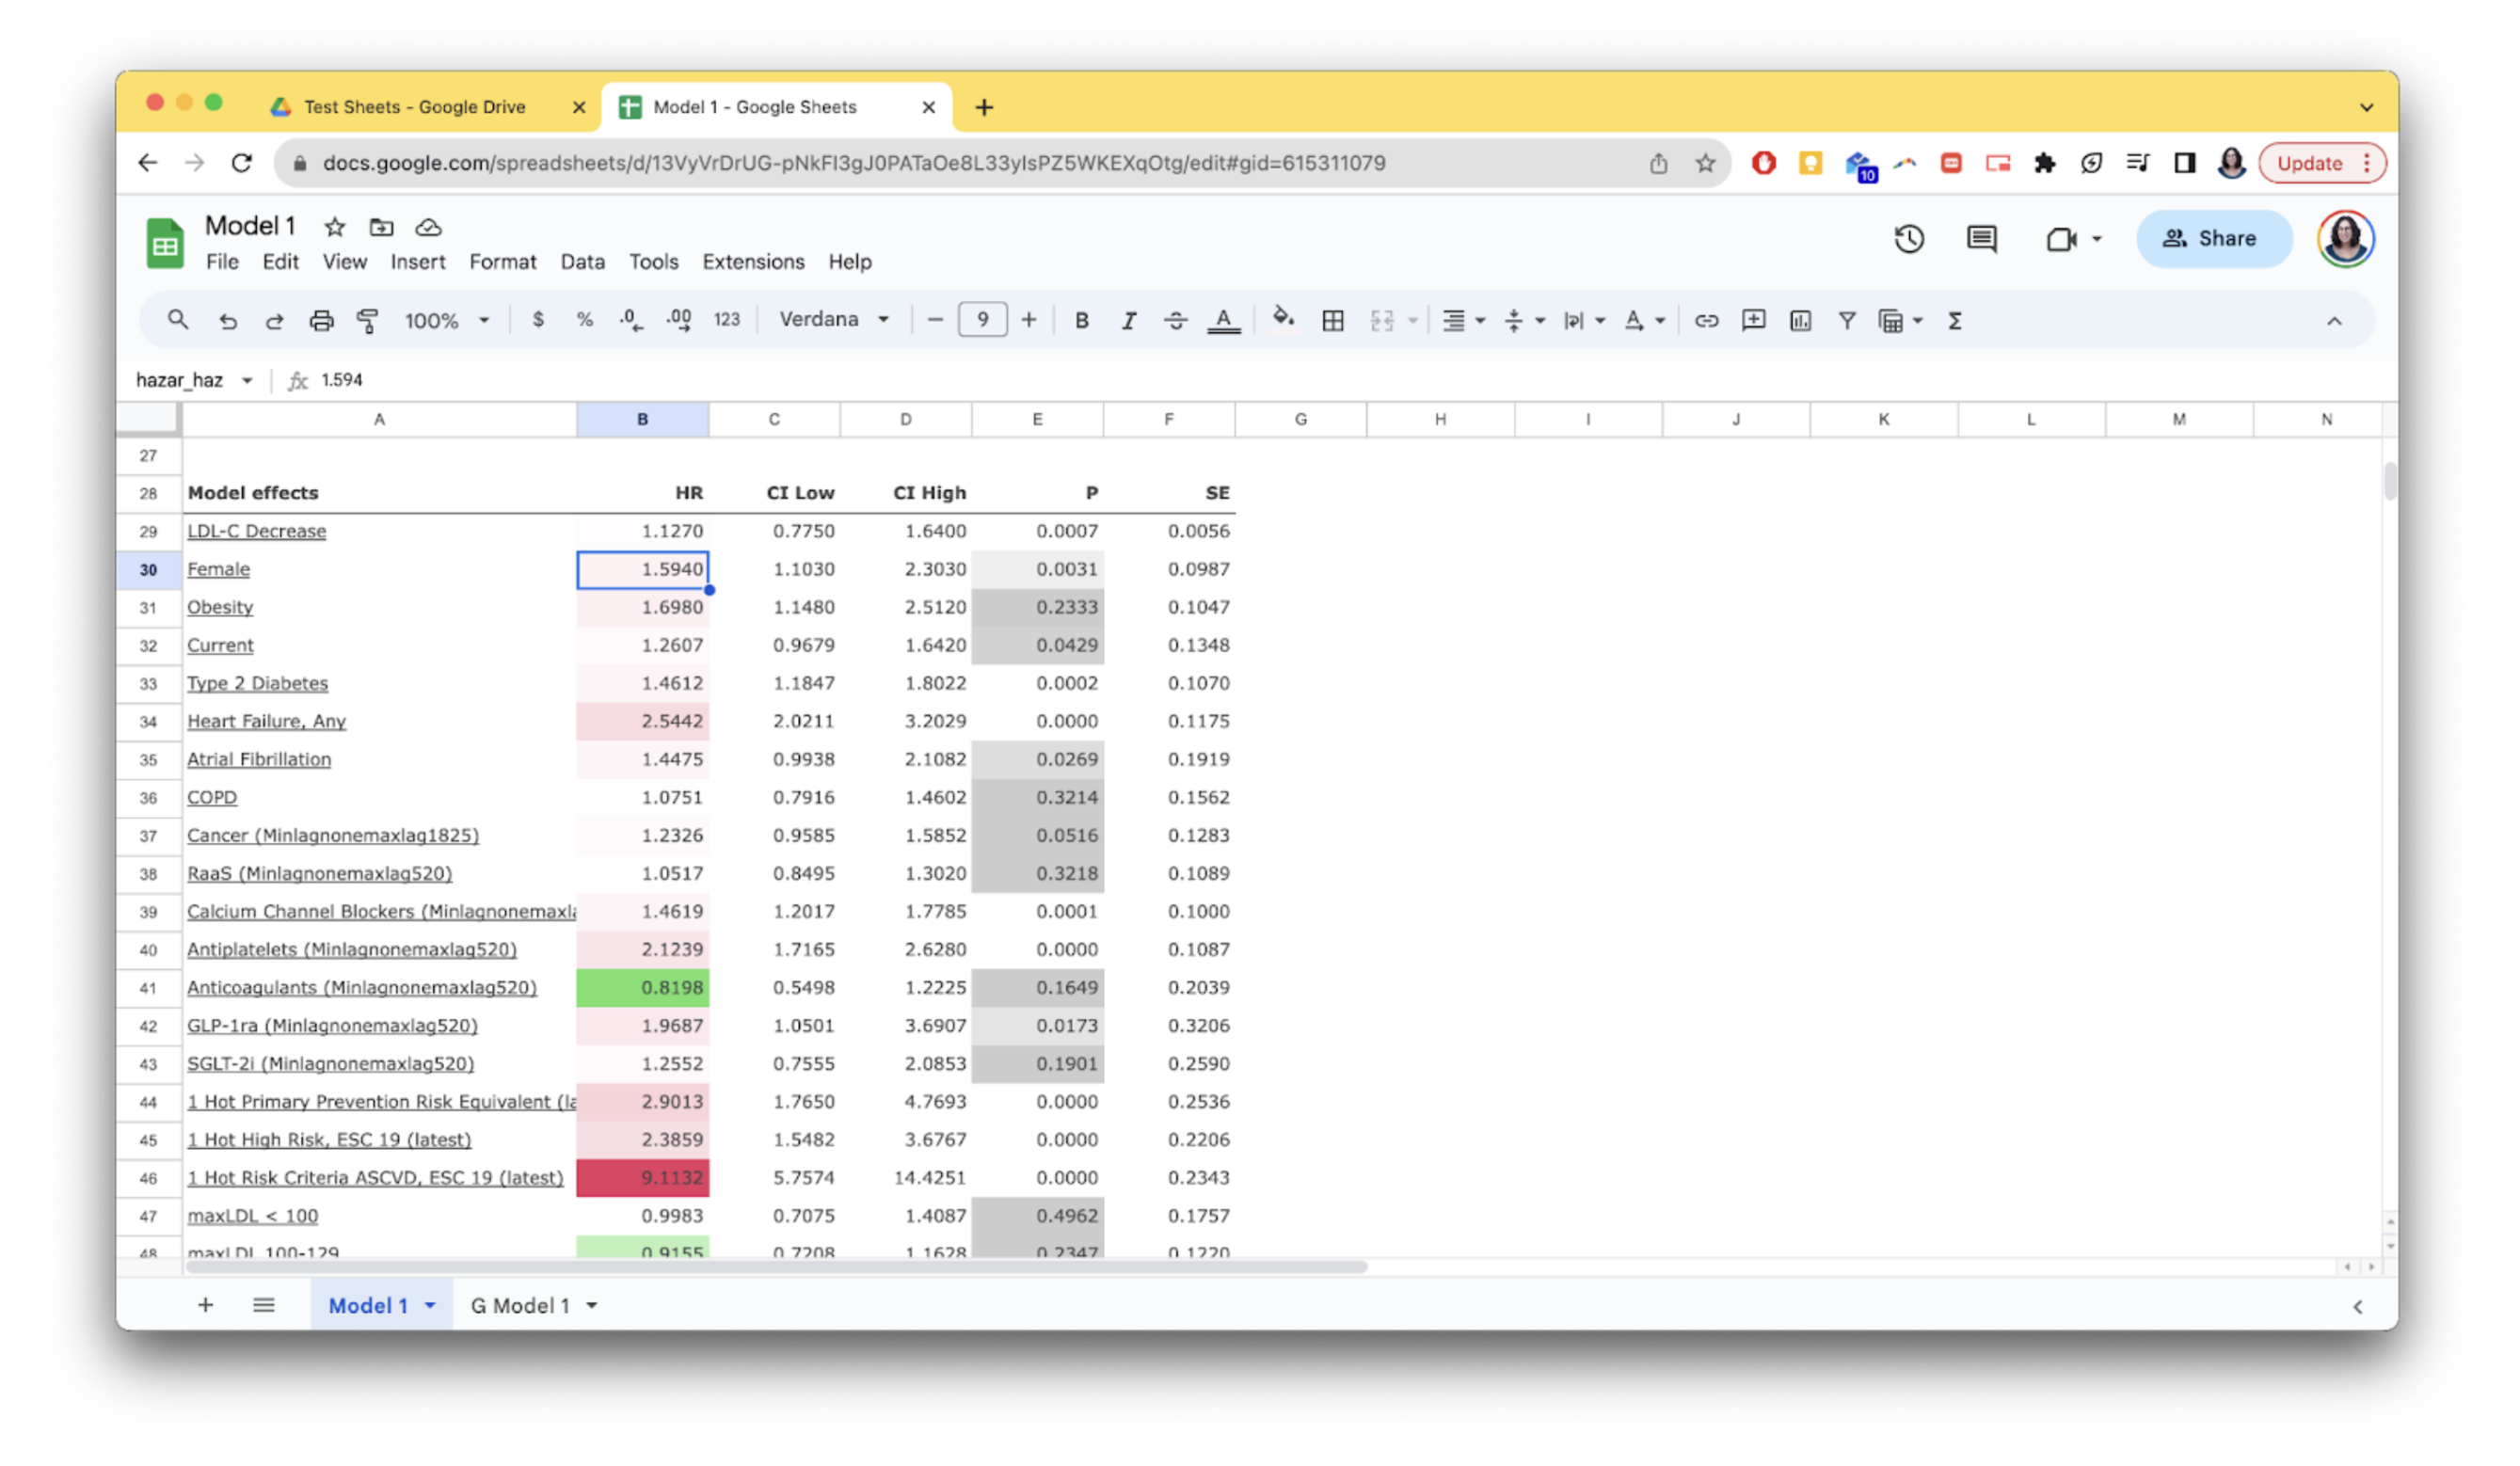
\includegraphics[width=\textwidth]{media/fig14.png}
  \caption{Spreadsheet Content for Cox Proportional Hazards Model 1 of
  the example.}
  \label{fig:ss}
\end{figure}

\subsection{Stage 2: Chart
Configuration}\label{stage-2-chart-configuration}

Once the data is retrieved and prepared, the next step involves defining
the chart specifications. For our example, we aim to visualize the
metrics from the Cox Proportional Hazards Models in the form of a Forest
Plot. VV library allows this by leveraging Vega-Lite, a high-level JSON
syntax for generating visualizations.

To accomplish this, the ForestPlot class is employed. This class is a
concrete implementation that inherits from AbstractChartNotationBuilder.
It specializes in constructing Forest Plots by setting the necessary
parameters, configurations, and data values. Moreover, the
ForestPlotBinding class plays a vital role. This class inherits from
AbstractChartNotation and is designed to hold and resolve the data
points essential for a Forest Plot.

The JSON configuration for our Forest Plot, generated by the
aforementioned classes, includes specific elements that are essential
for visualizing the hazard ratios and their corresponding confidence
intervals for the listed covariates (see Listing \ref{listing:14}). The JSON file lays
out not only the type of chart to be generated but also fine-grains the
aesthetic details such as titles, subtitles, and axes properties.

The configuration also takes advantage of Vega-Lite\textquotesingle s
layering capabilities. This enables us to represent multiple elements
like the confidence intervals and hazard ratios within the same plot
while maintaining visual coherence. Each metric, such as
\textquotesingle Age\textquotesingle,
\textquotesingle Sex\textquotesingle,
\textquotesingle Obesity\textquotesingle, etc., is represented as a
horizontal line in the Forest Plot, with markers indicating the
confidence interval and a point indicating the hazard ratio. For this
example we will use only three covariates.

\begin{code}
  \begin{minted}
    [
      frame=lines,
      framesep=2mm,
      baselinestretch=1.2,
      bgcolor=LightGray,
      linenos,
      breaklines
      ]
      {json}
{
  "$schema": "https://vega.github.io/schema/vega-lite/v5.json",
  "data": {
    "values": [
      {"measure": "LDL-C decrease", "lo": 1.127, "hr":0.775, "hi": 1.64},
      {"measure": "Age", "lo": 1.594, "hr": 1.103, "hi": 2.303},
      {"measure": "Female", "lo": 1.698, "hr":1.148, "hi":2.512}
    ]
  },
  "title": {
    "text": "Title 1",
    "fontSize": 12,
    "subtitle": "Subtitle 1"
  },
  "facet": {
    "row": {
      "field": "cohort",
      "header": {
        "labelAngle": 360,
        "labelFontSize": 10.5
      }
    }
  },
  "spec": {
    "encoding": {
      "y": {
        "field": "measure",
        "type": "nominal",
        "axis": {
          "labelFontSize": 10
        }
      },
      "x": {
        "type": "quantitative",
        "axis": {
          "labelFontSize": 9
        }
      }
    },
    "layer": [
      {
        "mark": {
          "type": "rule"
        },
        "encoding": {
          "x": {
            "field": "lo"
          },
          "x2": {
            "field": "hi"
          }
        }
      }
      // Additional layers truncated for brevity
    ]
  },
  "config": {
    "background": "#F7F7F7",
    "font": "Barlow, Lato, Roboto, sans-serif"
  }
}
  \end{minted}
  \caption{JSON Configuration for Forest Plot.}
  \label{listing:14}
  \end{code}

\subsection{Stage 3: Chart Rendering}\label{stage-3-chart-rendering}

With the data properly set and the chart configuration in place, we are
now ready to render the Forest Plot. To achieve this, we make use of
altair-save, an external package that integrates with our architecture.

The core class responsible for this task is AltairChartRenderer, which
extends the AbstractChartRenderer. This specialized class serves as a
wrapper for Vega-Altair, utilizing the Altair library to perform the
rendering of visualizations. In this architecture, the
AltairChartRenderer takes the JSON configuration produced by ForestPlot
and ForestPlotBinding classes and uses it to generate the visual
representation of the Forest Plot.

In most of our workflows, the AltairChartRenderer outputs a file pointer
(fp), typically an in-memory file-like object such as a StringIO object.
This allows for easy manipulation and further use of the chart in the
subsequent steps of deployment. However, the renderer is also flexible
enough to output the chart as a saved image file, supporting various
formats like SVG, for example.

In Figure \ref{fig:forest}, you will find a sample of what the rendered Forest Plot
looks like.

\begin{figure}[ht]
  \centering
  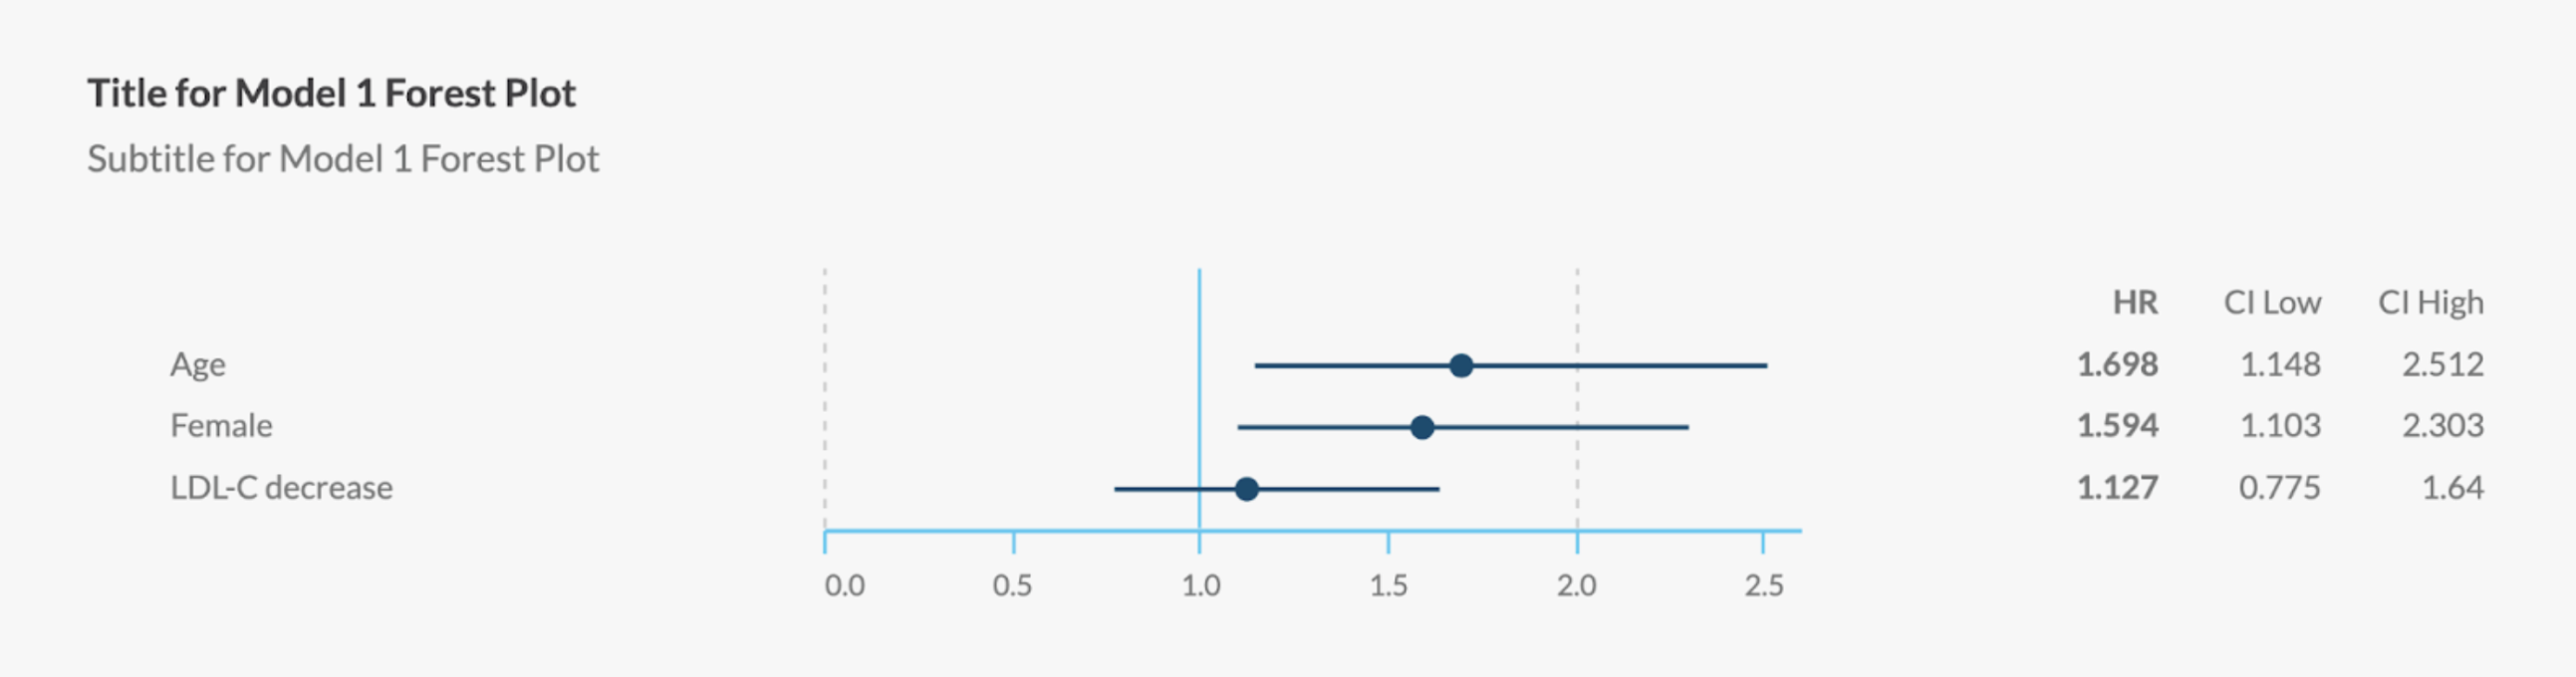
\includegraphics[width=\textwidth]{media/fig15.png}
  \caption{Rendered Forest Plot for Model 1 of the example.}
  \label{fig:forest}
\end{figure}

\subsection{Stage 4: Deployment}\label{stage-4-deployment}

The final stage of the workflow involves deploying the rendered Forest
Plot to a Miro board and Google Drive. To achieve this, the VV library
employs the specialized classes MiroBoardDeployer and
GoogleDriveDeployer.

Both classes automatically handle the upload process, ensuring that the
visualizations are transferred to their designated platforms. This
streamlined approach makes the visualizations readily accessible for
team collaboration (see Figure\ref{fig:forest_svg}).

\begin{figure}[ht]
  \centering
  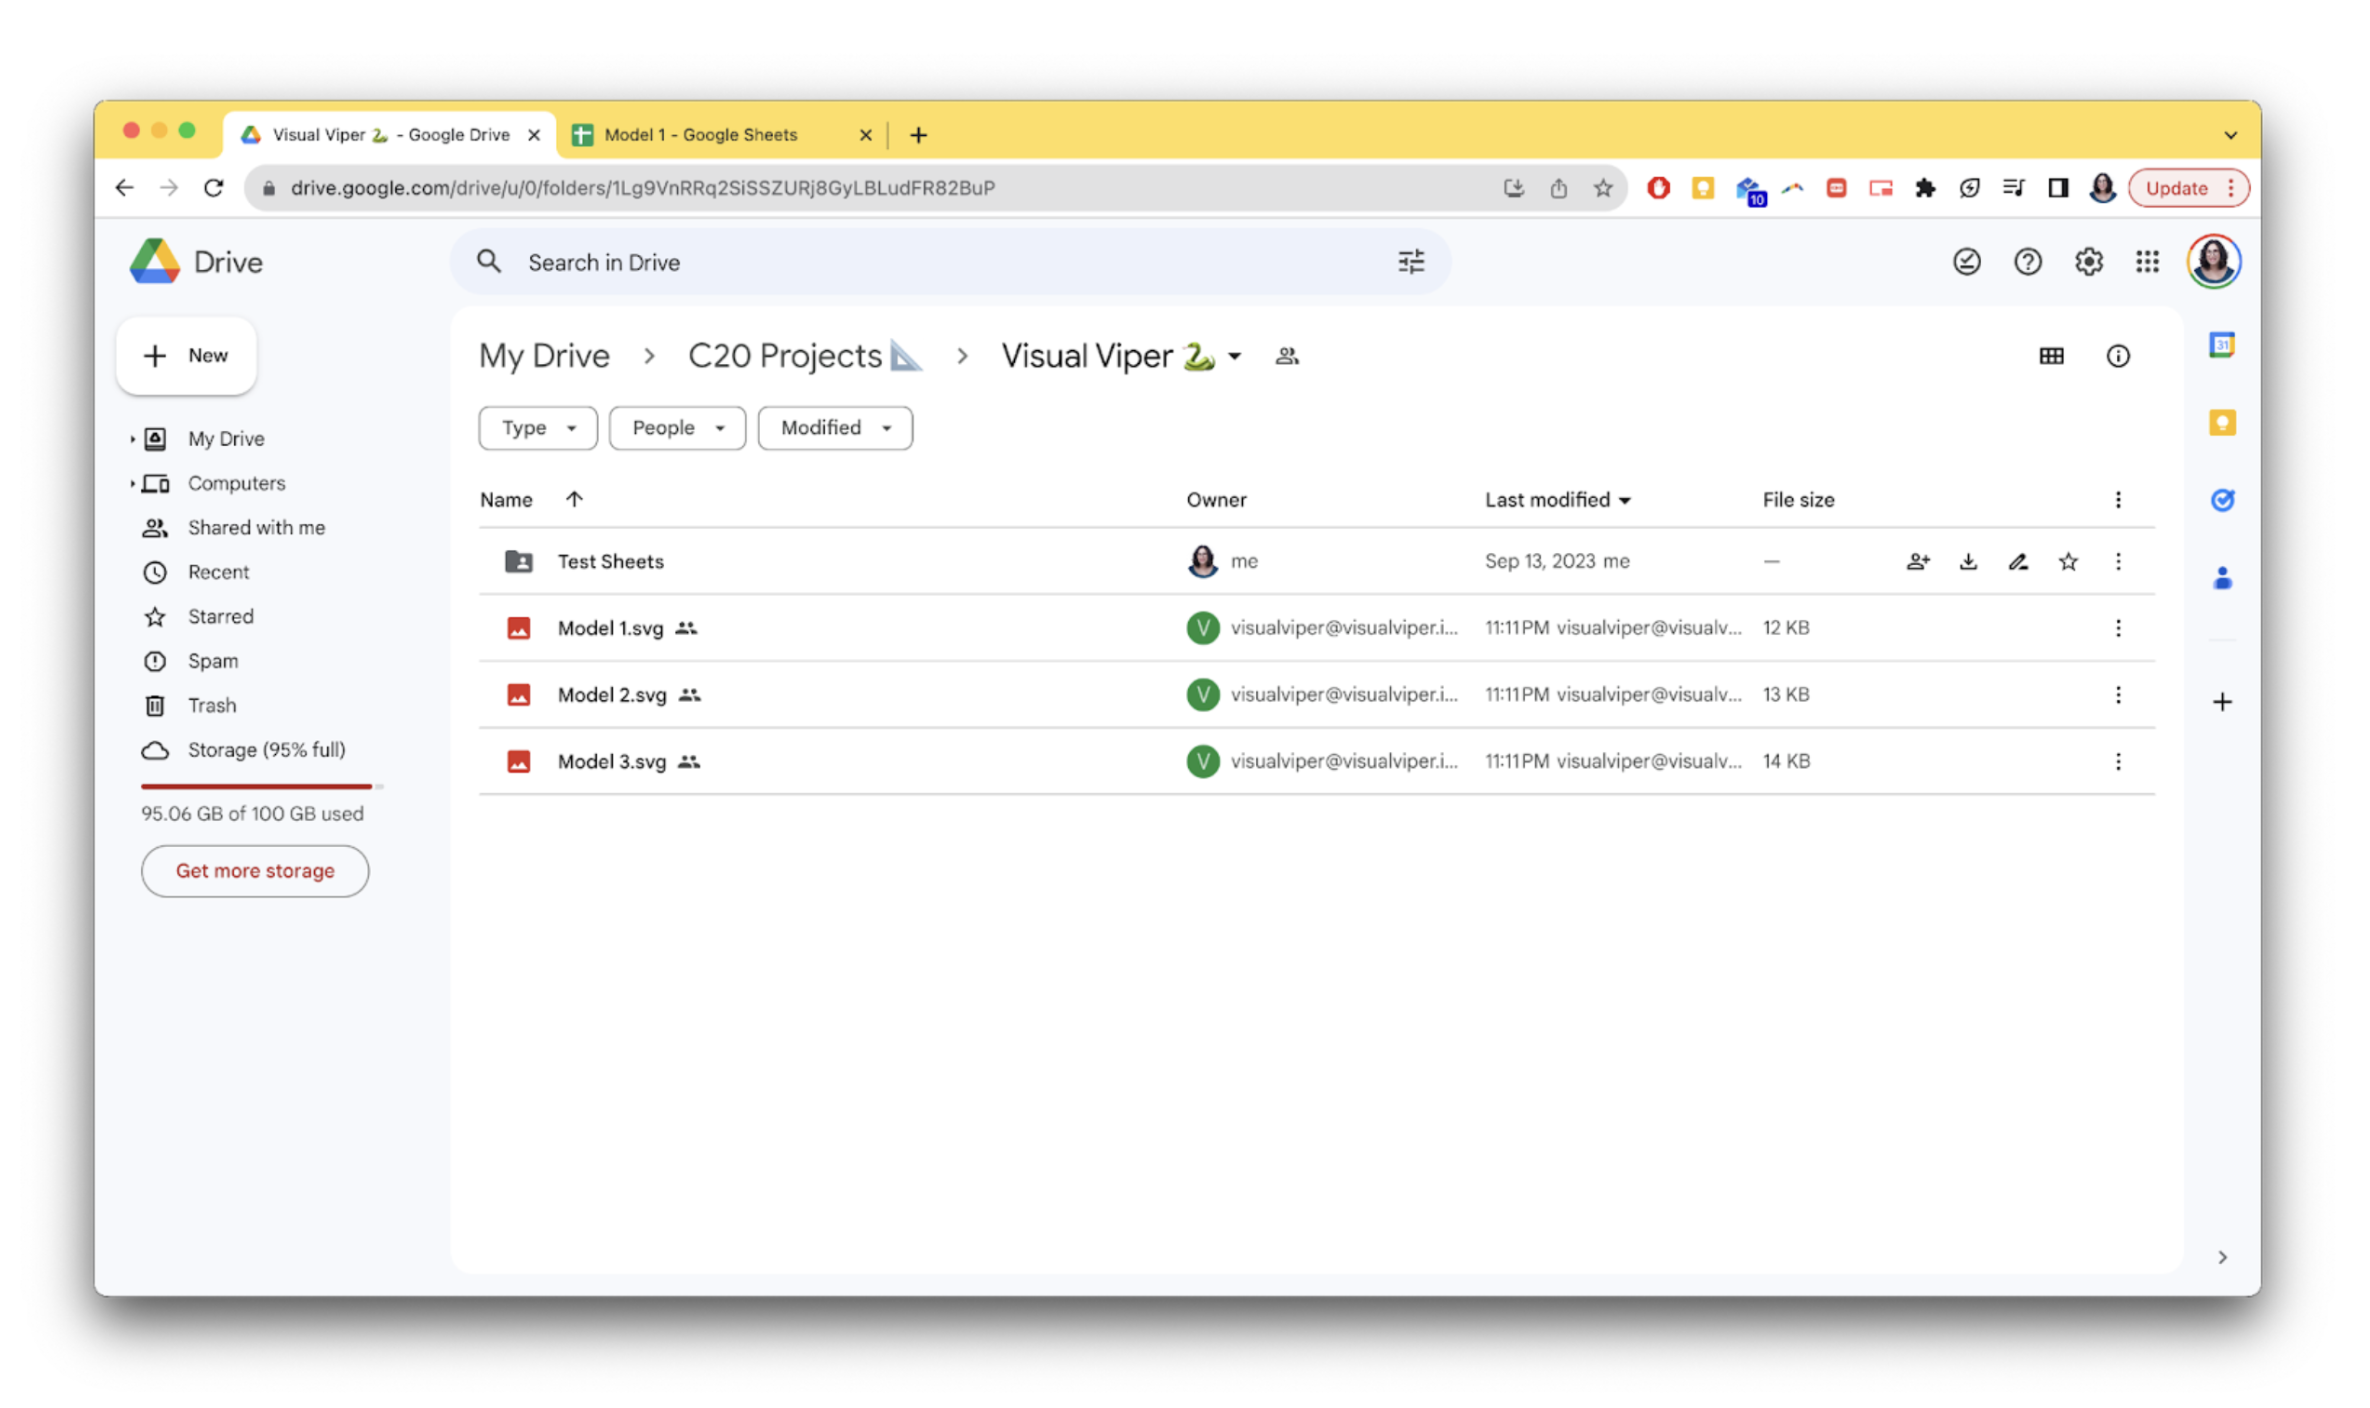
\includegraphics[width=\textwidth]{media/fig16.png}
  \caption{Forest plot SVG files on Google Drive, uploaded by the Visual Viper agent.}
  \label{fig:forest_svg}
\end{figure}


When deploying to a Miro board, the MiroBoardDeployer class offers
additional layout capabilities. Specifically, it arranges the Forest
Plots in a grid formation based on a user-defined number of columns. In
our example, the Forest Plots are laid out in a two-column grid,
facilitating a visually organized comparison of different plots (see
Figure \ref{fig:forest_miro1}).

For more extensive projects that require the deployment of a large
number of Forest Plots, the MiroBoardDeployer is equally capable. It can
layout tens of plots on the Miro board in an organized grid, allowing
for seamless interpretation and analysis of a more extensive data set
(see Figure \ref{fig:forest_miro2} for a different example of Forest Plots deployed in Miro
with tens of plots).

\begin{figure}[ht]
  \centering
  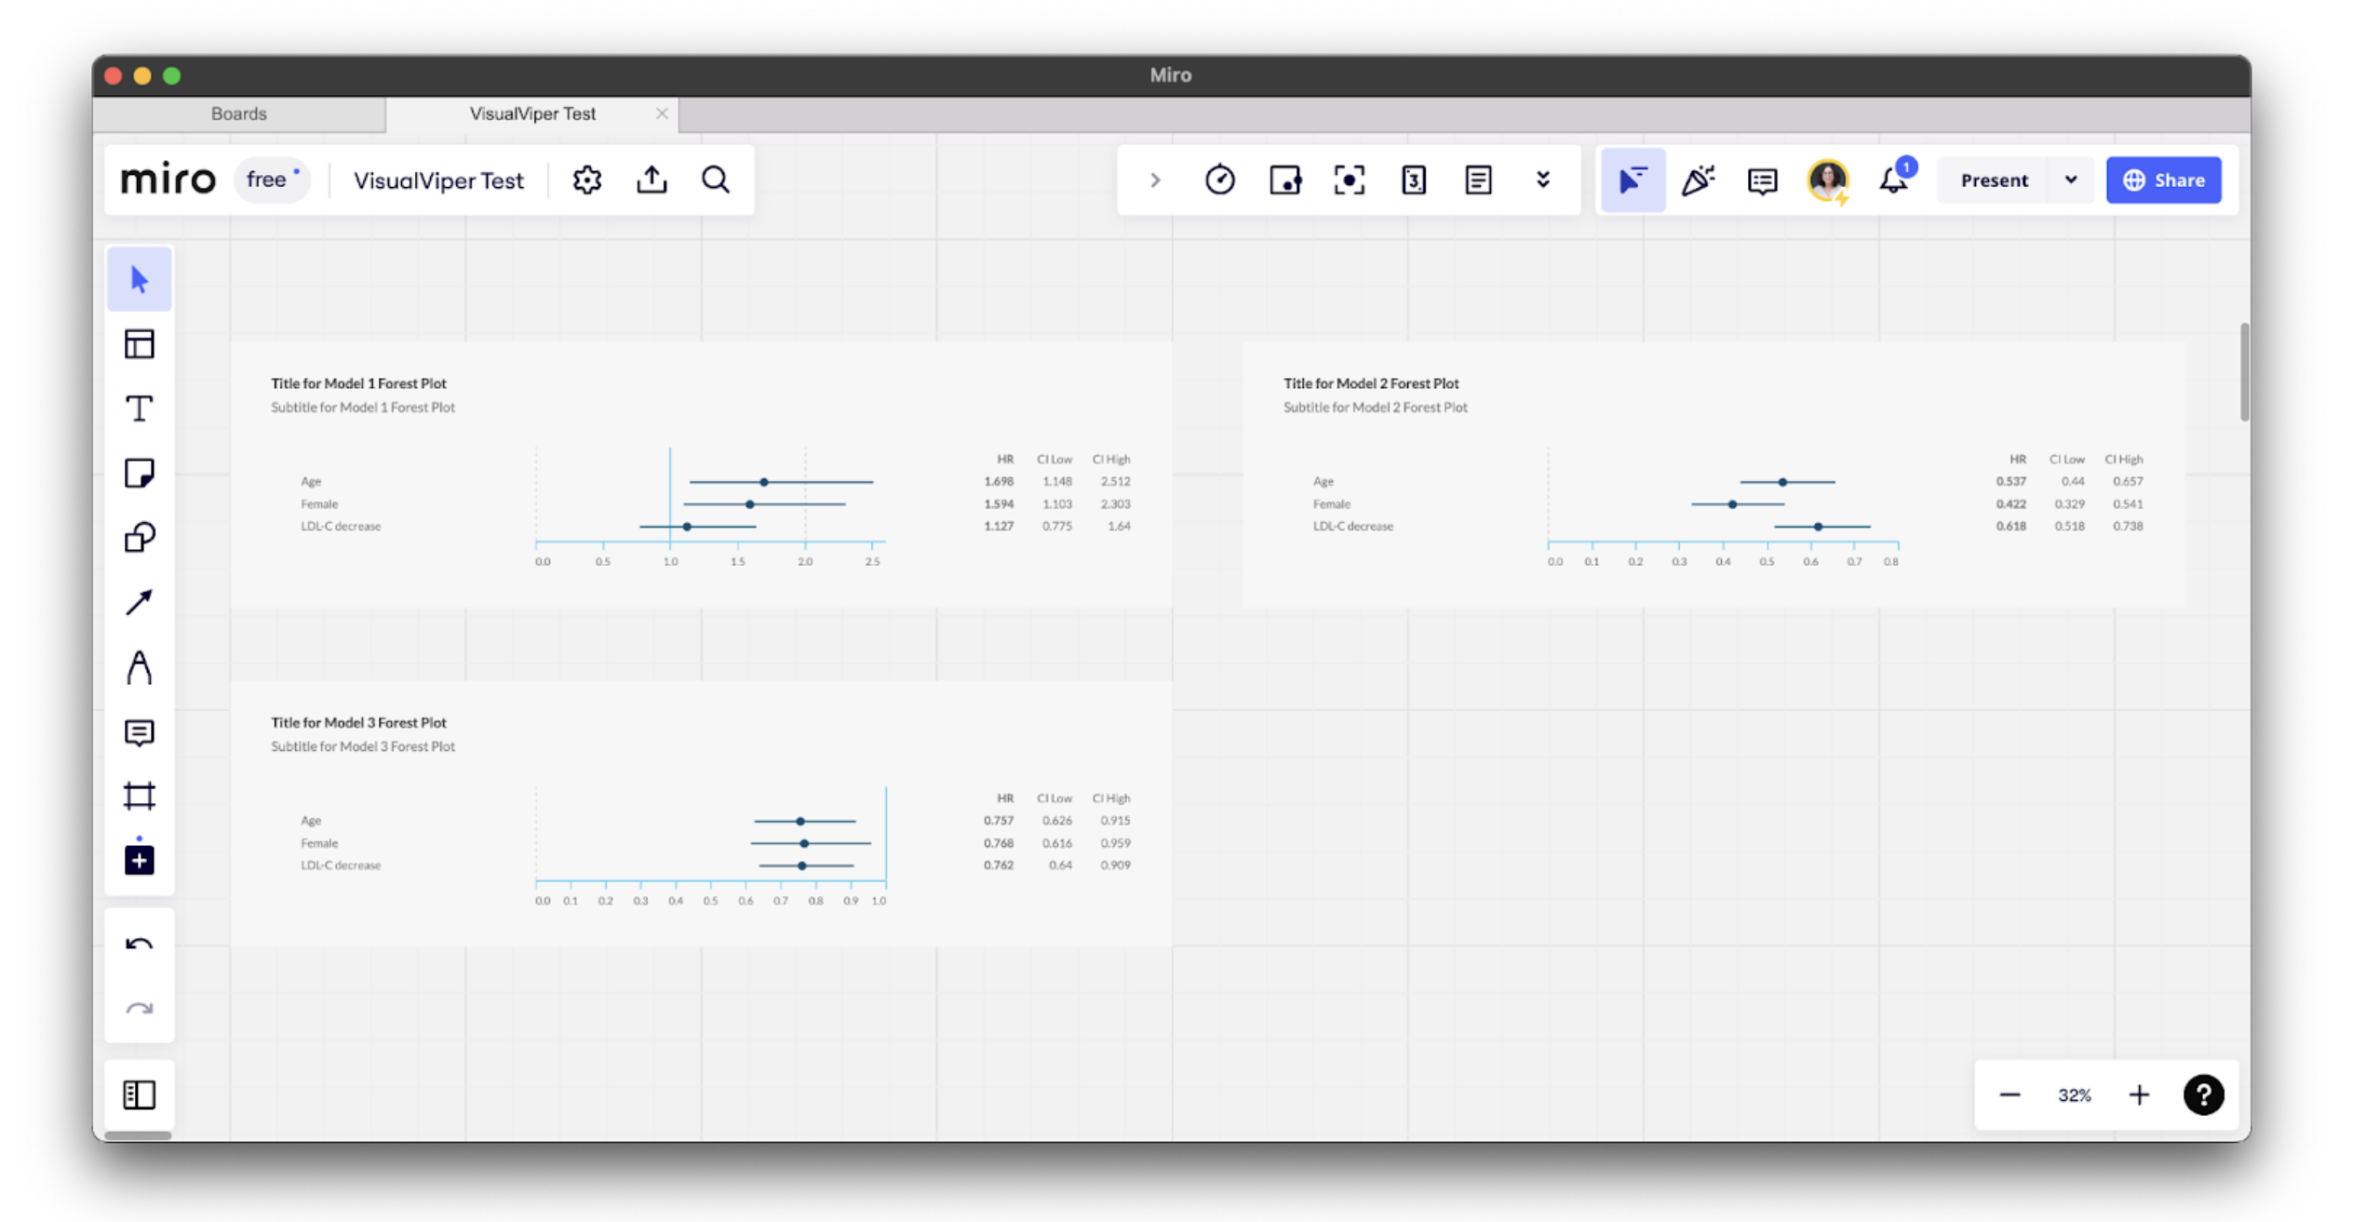
\includegraphics[width=\textwidth]{media/fig17.png}
  \caption{Forest Plots for Models 1-3 of the example on Miro Board.}
  \label{fig:forest_miro1}
\end{figure}

\begin{figure}[ht]
  \centering
  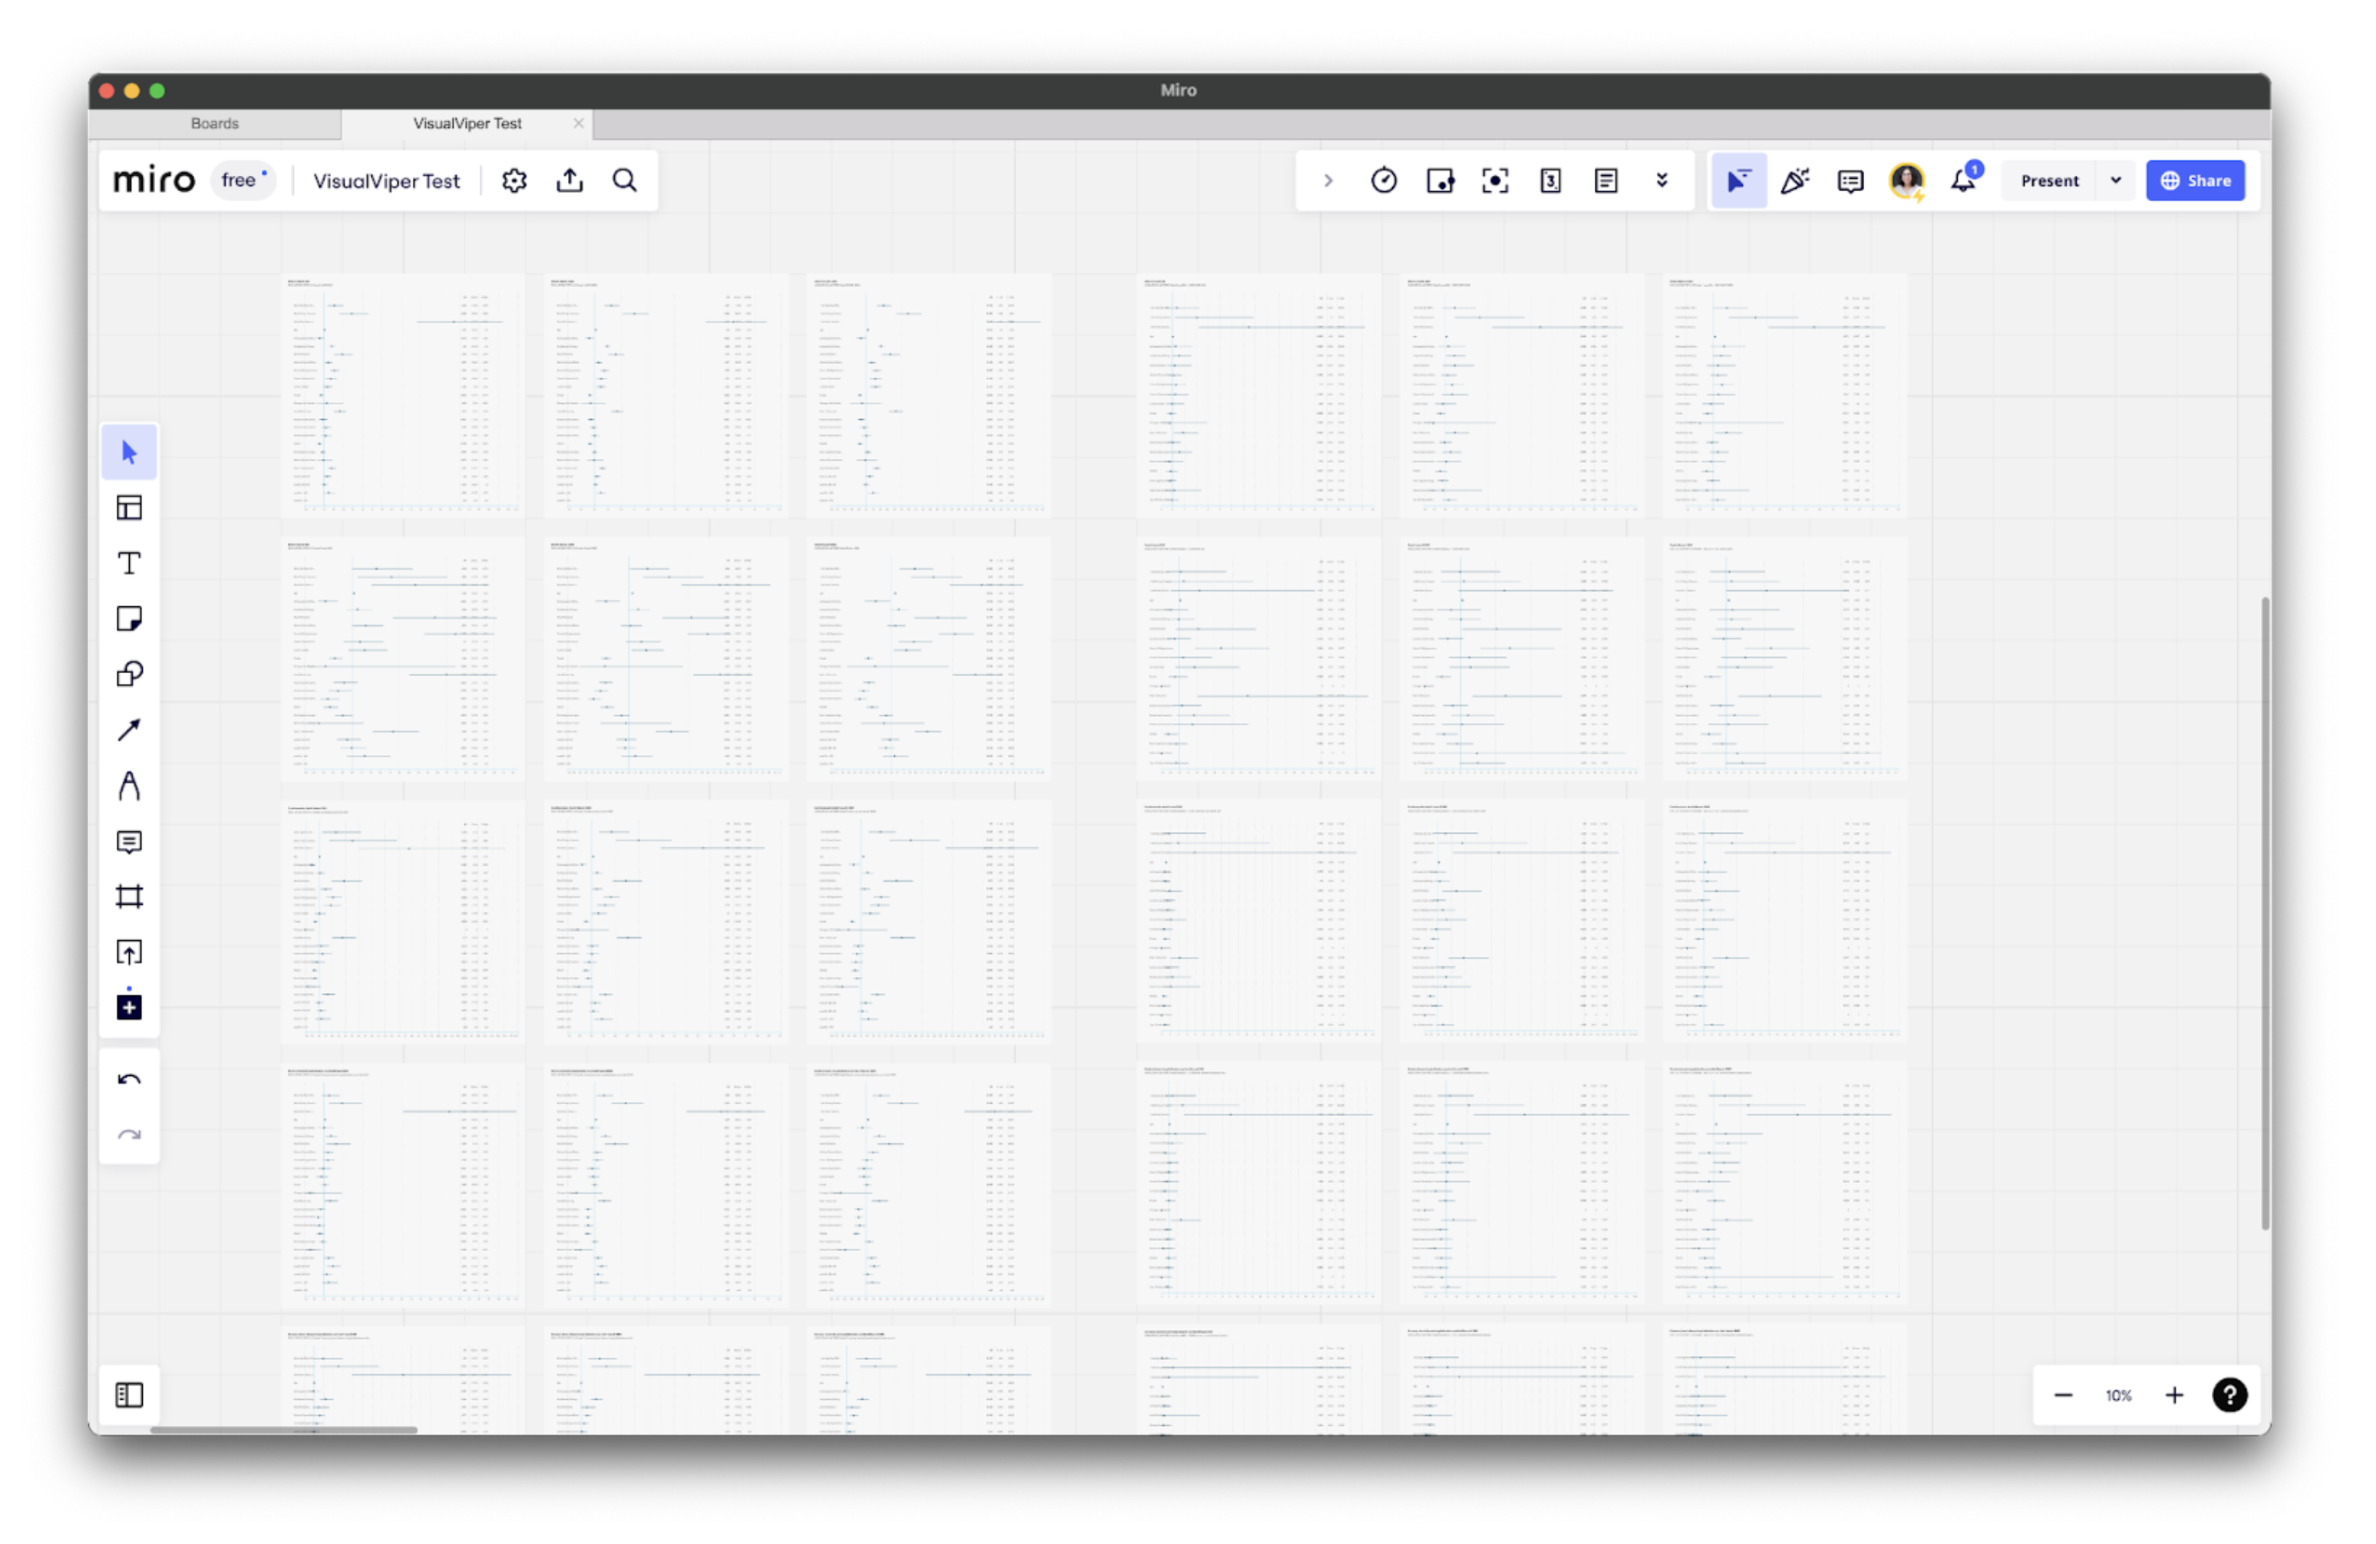
\includegraphics[width=\textwidth]{media/fig18.png}
  \caption{Different example of Forest Plots deployed in Miro with tens
  of plots laid out in a grid.}
  \label{fig:forest_miro2}
\end{figure}
